\chapter{Mathematical Modelling}\label{ch:mathmodel} 
\todo[color=04mathematicalModelling,inline]{Mathematical Modelling}
Most physical systems can be modelled statically or dynamically.
Depending on the application of the model,
and therefore on the end goal of the controller,
either option has some benefits and flaws.

Since our focus shifted during the project, we started out developing a static model,
describing the steady state response of the system.
Later on we decided to move towards a dynamic model, for easier PID-controller development.

Both modelling processes are described in this chapter.


\section{Static Modelling}\label{sec:statmod}
The static model explains the behaviour of the system at steady-state,
i.e. when the output is settled after a step input.
Static models are therefore also referred to as steady-state models.
Both expressions are used interchangeably throughout this report.

Typical static models for pump systems are pump curves and system curves.
%\todo[color=04mathematicalModelling,inline]{explain differences between pump curves and system curves}
%\todo[color=04mathematicalModelling,inline]{make sure sections and subsection makes sense}

\newpage
We used the data gathered through experiments to develop a model that would fit all our data,
within a certain degree of error,
\todo[color=04mathematicalModelling]{what is the degree?}
and around an operating point.
\todo[color=04mathematicalModelling]{what i the operation point?}
A model that could fit all the data without any error error would have to be of a very high order
and would probably model the system and sensor noise.

We decided to use grey-box modelling with polynomial fitting.
We consider our approach as grey-box rather than black-box,
because we chose the degrees of the polynomials based on known and tested physical relations.
\todo[color=04mathematicalModelling]{do we need the last sentence?}

A very similar modelling process was already successfully used by Pedersen and Yang 
\cite{YangMultiPump2008} on the same setup.
The choice of degree for the polynomials was determined by the affinity laws \cite{Volk2014}
and supported by very good fit to the data.

ML Curve Fitting Toolbox (\textit{cftool}) \cite{cftool}
was used in order to find the polynomial coefficients most accurately describing the system.

\subsubsection{Single Pump Model}
Equations \ref{eq:pumpHeadModel} and \ref{eq:pumpPowerModel} show a model that 
determines the head $H$ and the power $P$,
at a given flow $Q$ \cite{Yang2010}. 
Although the formula does not directly relate to the pump speed, it indirectly relates to it,
due to the fact that only one possible pump speed $\omega$ exists for a given flow,
provided the impeller diameter $D$ remains constant (compare \ref{sub:afflaws}).


\begin{equation}
	H = \bar{a_{2}} \cdot Q^2 + \bar{a_{1}} \cdot Q + \bar{a_{0}}
	\label{eq:pumpHeadModel}
\end{equation}
\begin{equation}
	P = \bar{b_{3}} \cdot Q^3 + \bar{b_{2}} \cdot Q^2 + \bar{b_{1}} \cdot Q + \bar{b_{0}}
	\label{eq:pumpPowerModel}
\end{equation}

The coefficients are determined by the pump characteristics and can be experimentally identified.
Taking variable speed into account, the equations \ref{eq:pumpHeadModel}  and \ref{eq:pumpPowerModel}
will depend on the motor speed\cite{Yang2010}. The pump Affinity Laws state:

\begin{align*}
	\left(\frac{\omega_1}{\omega_2}\right)^1 = \frac{Q_1}{Q_2} && 
	\left(\frac{\omega_1}{\omega_2}\right)^2 = \frac{H_1}{H_2} &&
	\left(\frac{\omega_1}{\omega_2}\right)^3 = \frac{P_1}{P_2}		
\end{align*}\cite{Volk2014}.

Assuming the pump model parameters ($\bar{a_{0}}$, $\bar{a_{1}}$, $\bar{a_{2}}$ and $\bar{b_{0}}$,
$\bar{b_{1}}$, $\bar{b_{2}}$, $\bar{b_{3}}$) described in equation \ref{eq:pumpHeadModel} and 
\ref{eq:pumpPowerModel} are obtained at a certain speed $\bar{\omega_{0}}$, 
this results in the following equation describing the pump at any speed $\omega$ \cite{Yang2010}.

\begin{equation}
	H(\omega) = a_0 \cdot \omega^2 + a_1 \cdot \omega \cdot Q(\omega) + a_2 \cdot Q(\omega)^2
	\label{eq:pumpHeadModel2}
\end{equation}
\begin{equation}
	P(\omega) = b_0 \cdot \omega^3 + b_1 \cdot \omega^2 \cdot Q(\omega) + b_2 \cdot \omega \cdot Q(\omega)^2 + b_3 \cdot Q(\omega)^3
	\label{eq:pumpPowerModel2}
\end{equation}

\newpage
The coefficients can be determined as follows:
\begin{align*}
	a_0 = \frac{\bar{a_0}}{\bar{\omega_0^2}} && a_1 = \frac{\bar{a_1}}{\bar{\omega_0}} && a_2 = \bar{a_2} \\
	b_0 = \frac{\bar{b_0}}{\bar{\omega_0^3}} && b_1 = \frac{\bar{b_1}}{\bar{\omega_0^2}} && b_2 = \frac{\bar{b_2}}{\omega_0} && b_3 = \bar{b_3}
\end{align*}
\cite{Yang2010}

As observed in equations \ref{eq:pumpHeadModel2} and \ref{eq:pumpPowerModel2} the coefficients are
initially multiplied by the input speed. Afterwards they are divided by the
speed they were determined for, in order to take into account the variable speed \cite{Yang2010}..

Figure \ref{fig:flowVsPressure} shows data points connected together that represent 
a pump head curve. As observed in the figure, when the opening percentage of the control valve is at
10\% the pressure seems to reach negative values. We believe, this arises from the fact that we were not 
able to properly calibrate the pressure sensors. As an alternative, we have used the gain and offsets
provided to us by previous researchers that have experimented on the same setup \cite{Jepsen2017}.
The gains and offsets that we were able to determine for Flow and Power Consumption,
respectively, were also consistent with the values determined by them.
This is the reason we decided to use the values provided to us.

\begin{figure}[h]
	\centering
	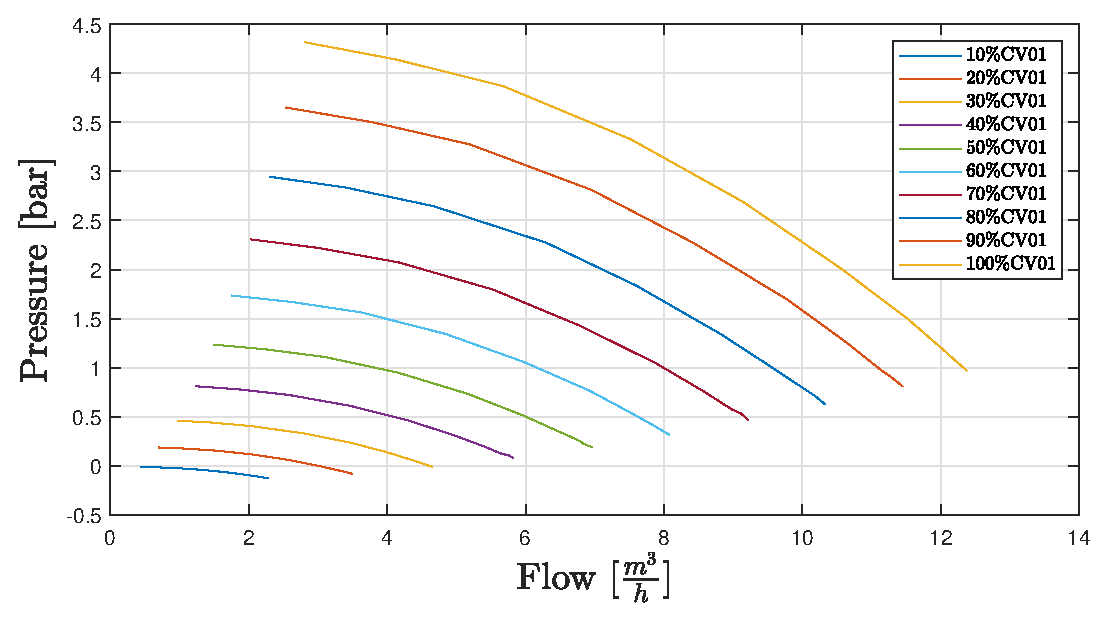
\includegraphics[width=1\textwidth]{figures/05mathematicalModelling/flowVsPressureRun34.eps}
	\caption{Data Points for Flow vs. Pressure}
	\label{fig:flowVsPressure}
\end{figure}

\newpage
Figure \ref{fig:flowVsPowerConsumption} shows data points connected together, representing a pump
power consumption curve.

\begin{figure}[ht]
	\centering
	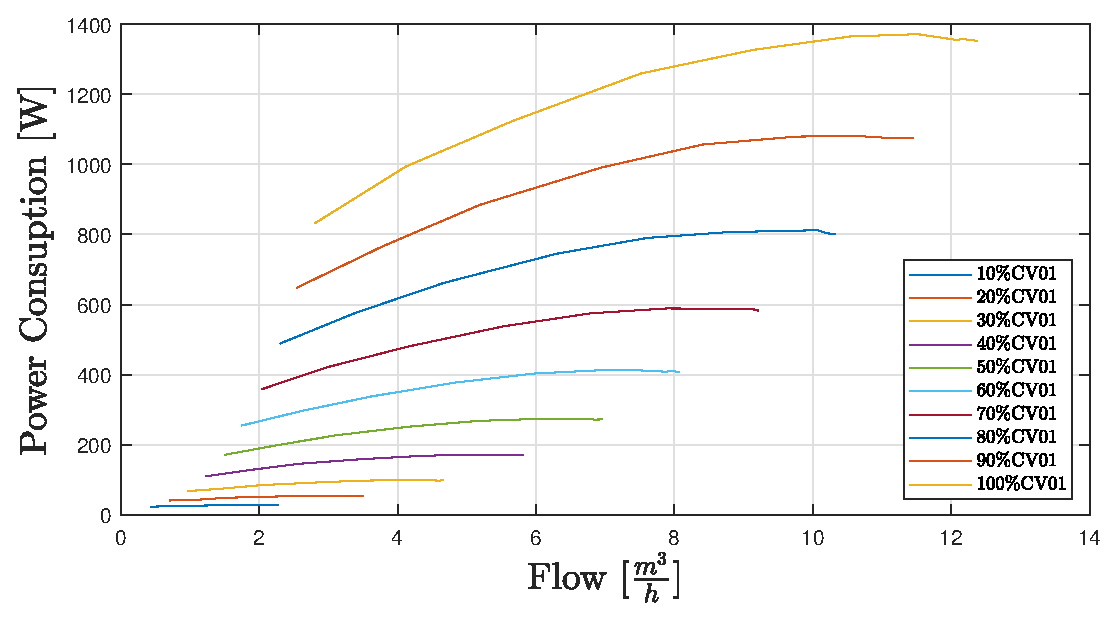
\includegraphics[width=1\textwidth]{figures/05mathematicalModelling/flowVsPowerRun34.eps}
	\caption{Data Points for Flow vs. Power Consumption}
	\label{fig:flowVsPowerConsumption}
\end{figure}

The ML tool \textit{cftool} \cite{cftool} was used to determine coefficients from each curve in  Figures 
\ref{fig:flowVsPressure} and \ref{fig:flowVsPowerConsumption}.

The coefficients for the model were determined at 60 \% pump speed, chosen at random and can be seen below.
\todo[color=04mathematicalModelling]{maybe not say at random, something to do with requirements possibly}
\begin{align*}
	a_0 = -0.03044 && a_1 = 0.07635  && a_2 = 1.688  \\
	b_0 = -0.2825 && b_1 = -0.7147 && b_2 = 54.39 && b_3 = 163.7 \\
\end{align*}
\newpage
\section{Dynamic Modelling}
Giving the system a unit step input, we determined the process reaction curve of the system. This has been used 
in order to calculate the PID coefficients when configuring the PID, using Zielger-Nichols tuning technique.
The next step was to model the curve, using equation \ref{eq:plantTransferFunction}.

\begin{equation}
	\frac{Y(s)}{U(s)} = \frac{A \cdot e^{-st_d}}{\tau \cdot s + 1}
	\label{eq:plantTransferFunction}
\end{equation}
\cite{Franklin2014}
\begin{itemize}
	\item A = final value the step response settles at
	\item $t_{d}$ = time delay
	\item $\tau$ = time it takes from 0.1 of final value to 0.9 final value
\end{itemize}

After analyzing the step response on the physical setup, we have determined the values to be A = 2.221, 
$t_d$ = 0.75 and $\tau$ = 2.62.

We have used ML to model the step response, and the result can be seen in Figure \ref{fig:modeledStepResponse}.

\begin{figure}[ht]
	\centering
	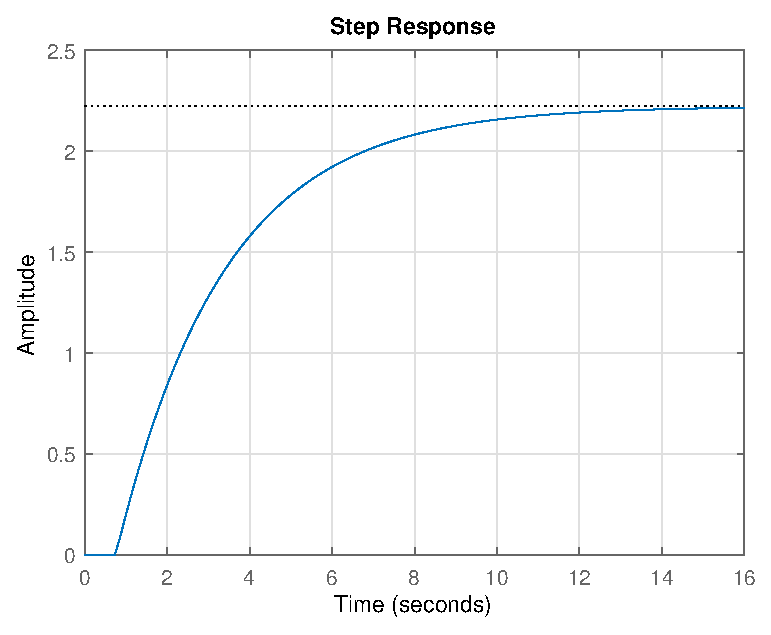
\includegraphics[width=0.8\textwidth]{figures/06ModelValidation/modeledStepResponse.eps}
	\caption{Modeled Step Response}
	\label{fig:modeledStepResponse}
\end{figure}

Important to notice, that the modeled step response looks quite accurate to the actual step response.
One key difference, would be the time delay. The unit step input is given instantly on the model,
while on the physical setup, there was a delay of 0.5 seconds, from the moment the simulation had started,
to the moment the unit step was given.
The next step was to implement the Ziegler-Nichols PID tuning method. The models obtained have been accurate
with some degree of error and they can be seen in Figure \ref{fig:modeledPI} and \ref{fig:modeledPID}.

\begin{figure}[ht]
	\centering
	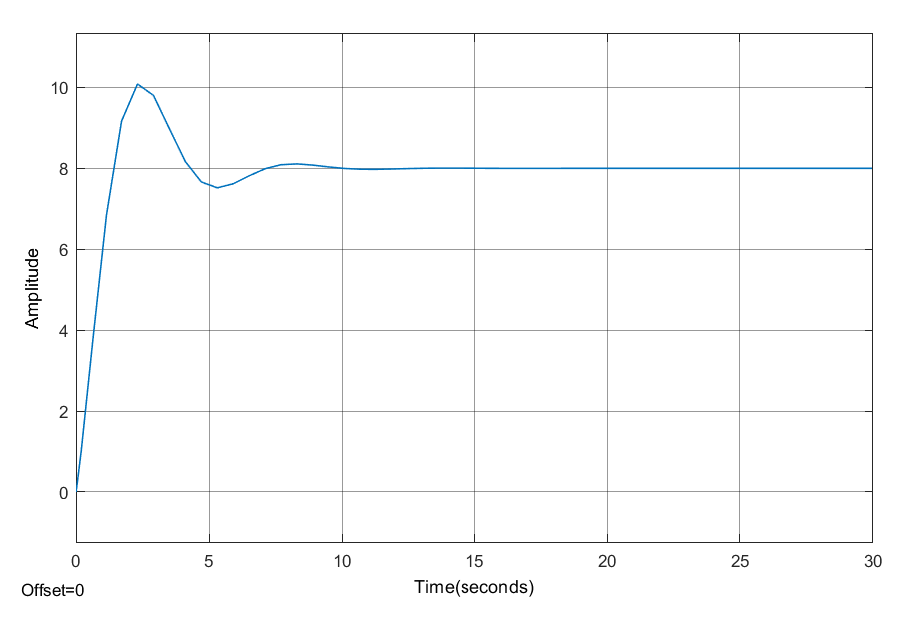
\includegraphics[width=0.7\textwidth]{figures/06ModelValidation/modelPI.eps}
	\caption{Modeled PI Controller}
	\label{fig:modeledPI}
\end{figure}
\vspace{-5mm}
\begin{figure}[ht]
	\centering
	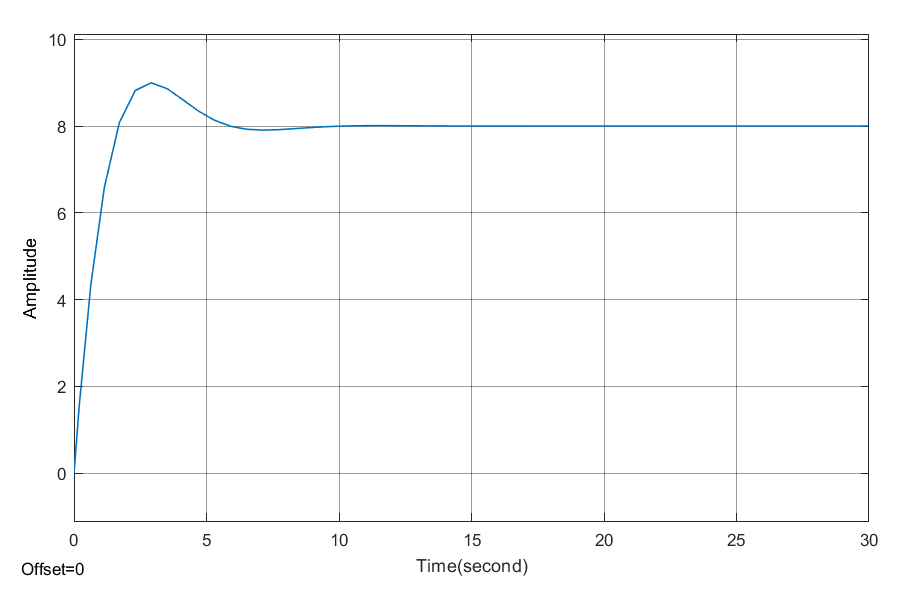
\includegraphics[width=0.7\textwidth]{figures/06ModelValidation/modelPID.eps}
	\caption{Modeled PID Controller}
	\label{fig:modeledPID}
\end{figure}

Both models predict with a relative high accuracy the  behavior of the physical setup, 
with a certain degree of error. Comparisons can be seen in Chapter \ref{ch:modValPerf} and Appendix \ref{app:modelling}.